\providecommand{\main}{../../../..}
\documentclass[\main/dresen_thesis.tex]{subfiles}

\begin{document}
  \section{GALAXI}\label{ch:appendix:lss:galaxi}
    \begin{figure}[h]
      \centering
      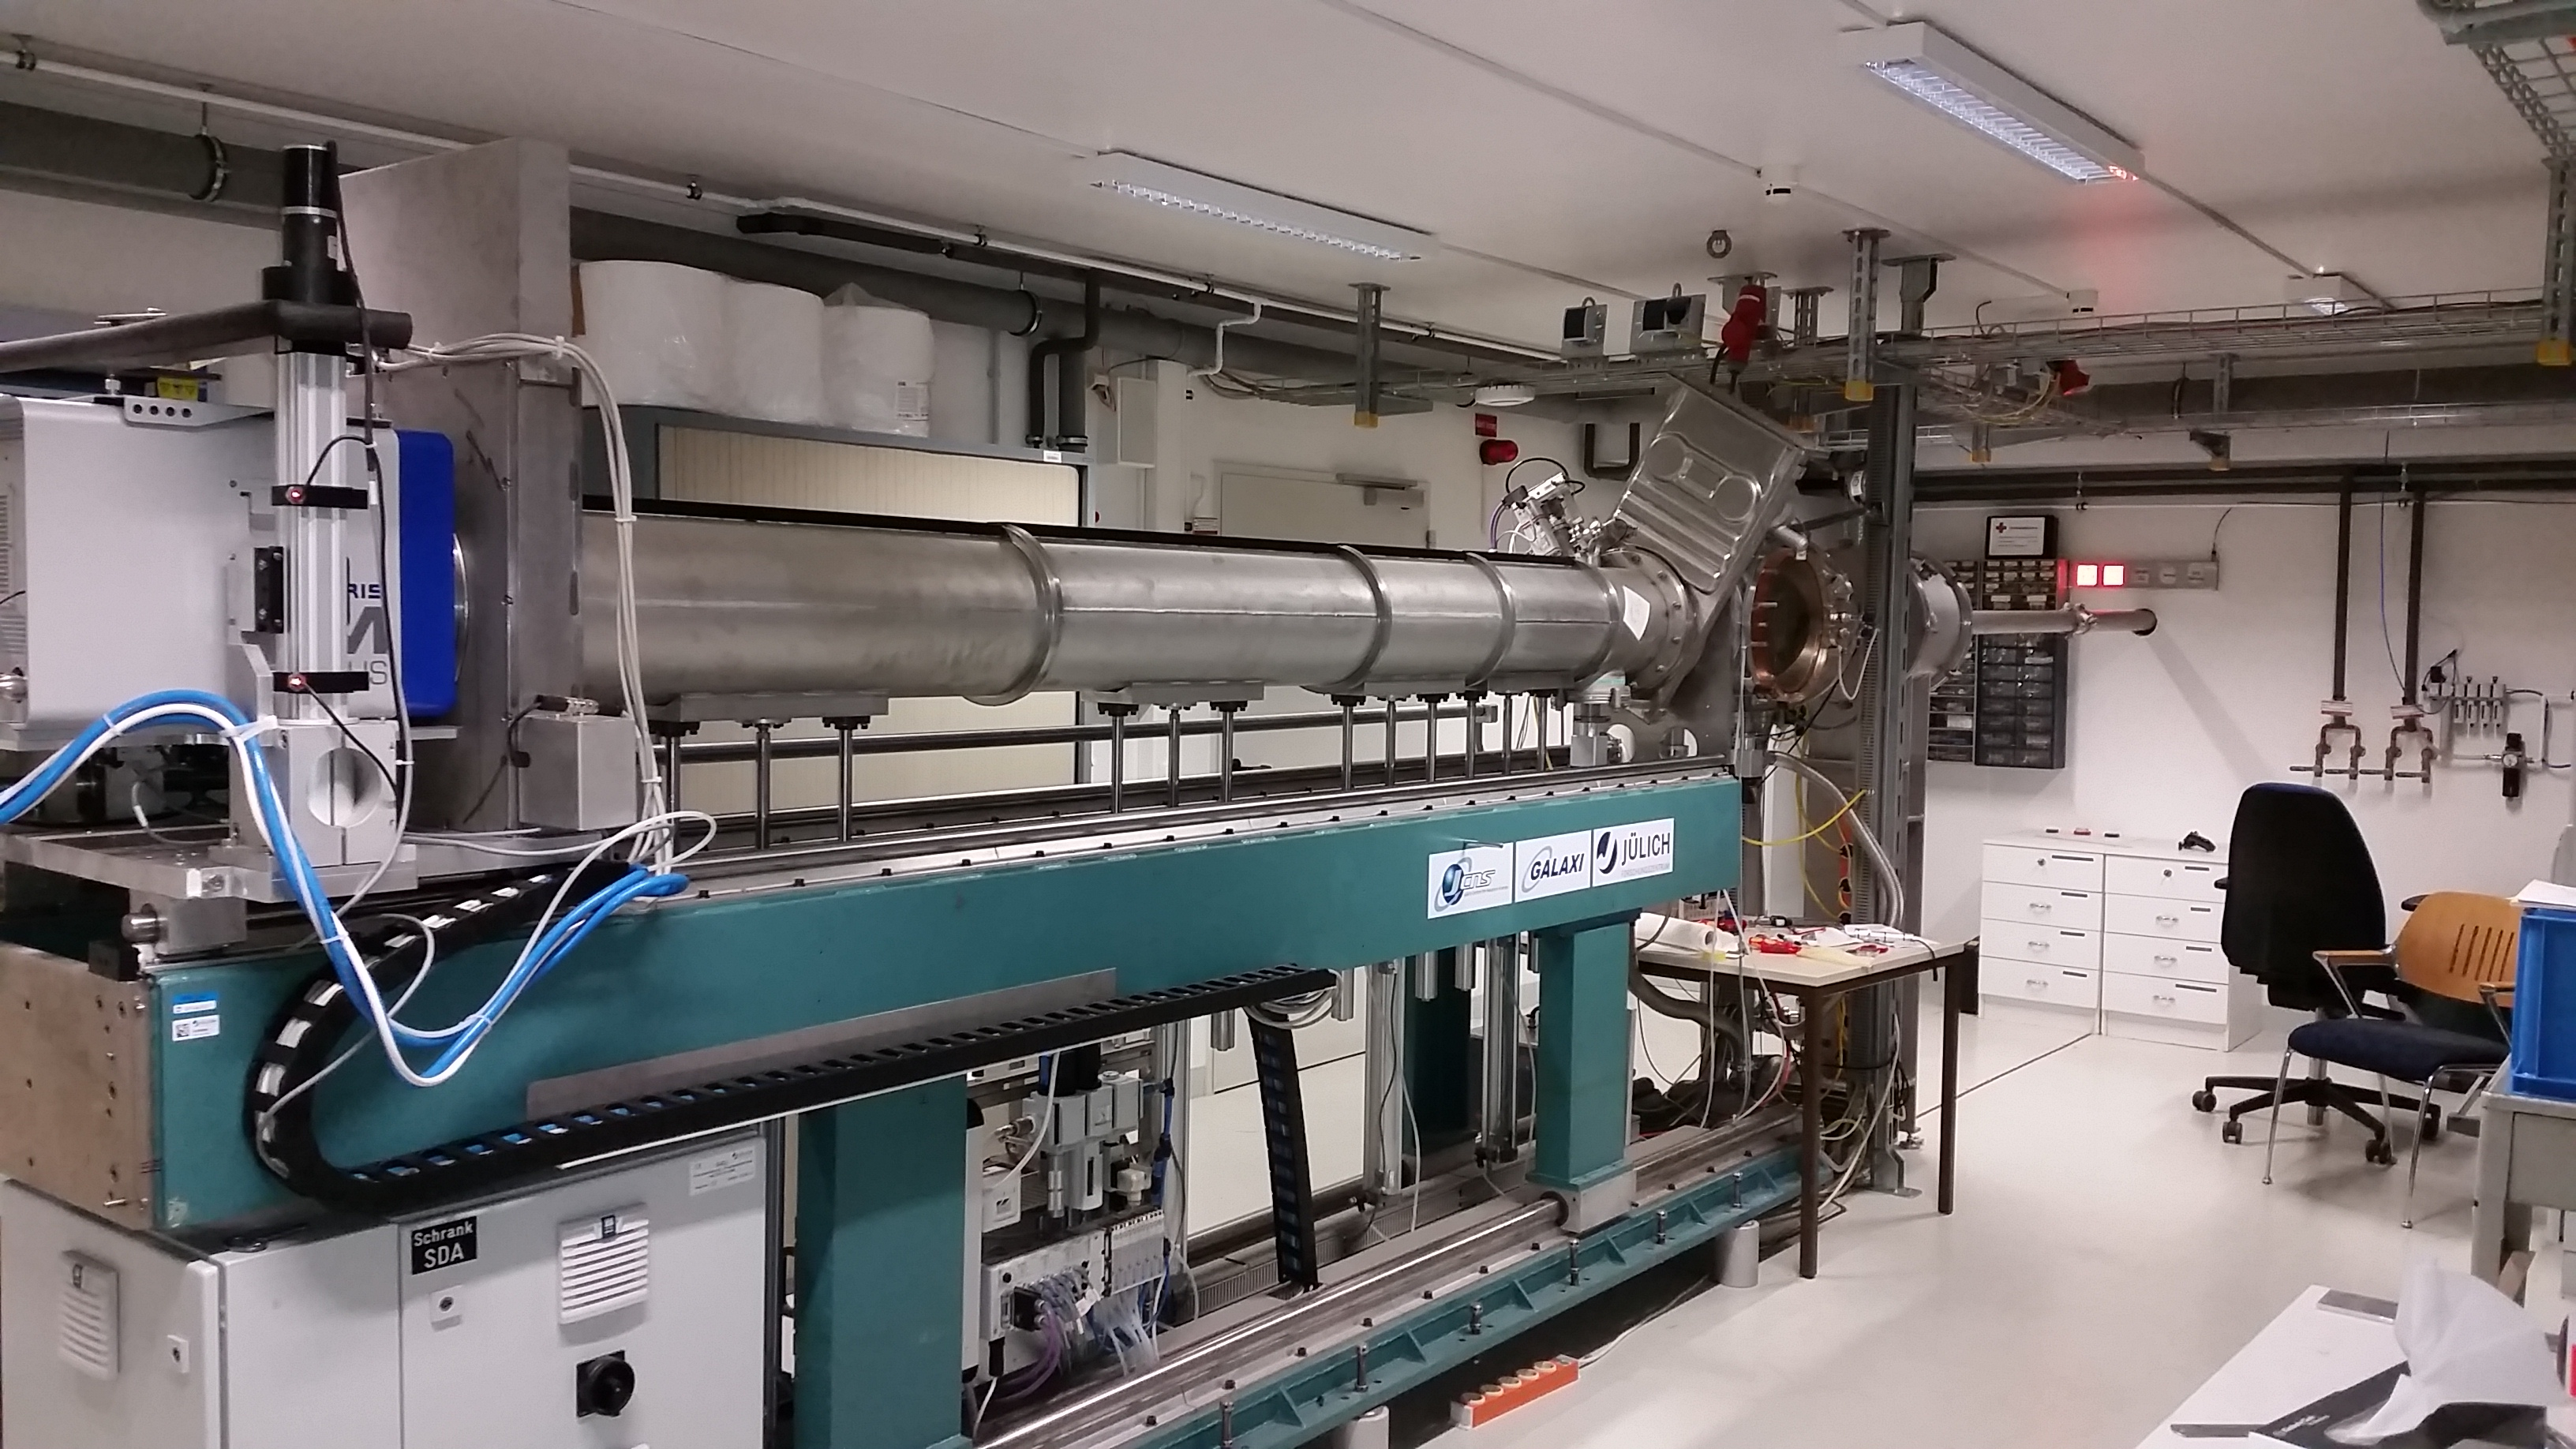
\includegraphics[width=0.7\textwidth]{instruments_galaxi}
      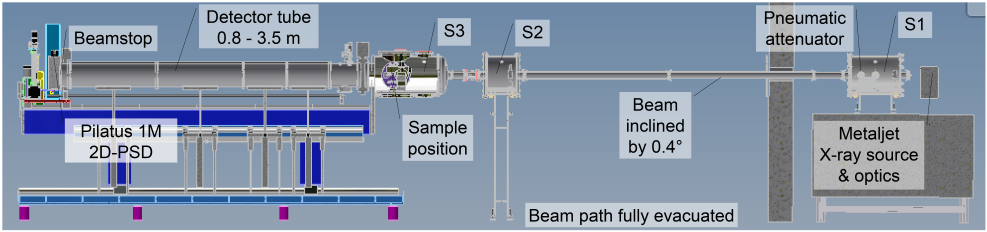
\includegraphics[width=0.7\textwidth]{appendix_instruments_GALAXISetup}
      \caption{\label{fig:appendix:lss:galaxi}GALAXI at Forschungszentrum J\"ulich, usable for (grazing incidence) small angle x-ray scattering and x-ray reflectometry.}
    \end{figure}

    The Gallium Anode Low-Angle X-ray Instrument (GALAXI) at the Forschungszentrum J\"ulich is set up with a liquid metal jet source and a position sensitive Pilatus 1M detector and can be used for (grazing incidence) small-angle x-ray scattering and x-ray reflectometry \cite{FZJ_2016_GALAX}.
    By using a circulating and continuously cooled metal jet of a GaInSn metal alloy, a high flux of x-ray photons is produced, comparable to a second generation synchrotron.
    The $K-\alpha$ wavelength is $\lambda \eq 1.34 \unit{\angstrom}$ and the sample-to-detector distance can be varied incrementally from $0.8 - 3.5 \unit{m}$.
    For the Pilatus 1M detector with a size of $169 \unit{mm} \times 179 \unit{mm}$ and pixel size of $172 \unit{\unitmu m}$ this results in a accessible q-range of $4 \cdot 10^{-2} \dots 8 \unit{nm}^{-1}$.

    \begin{figure}[h]
      \centering
      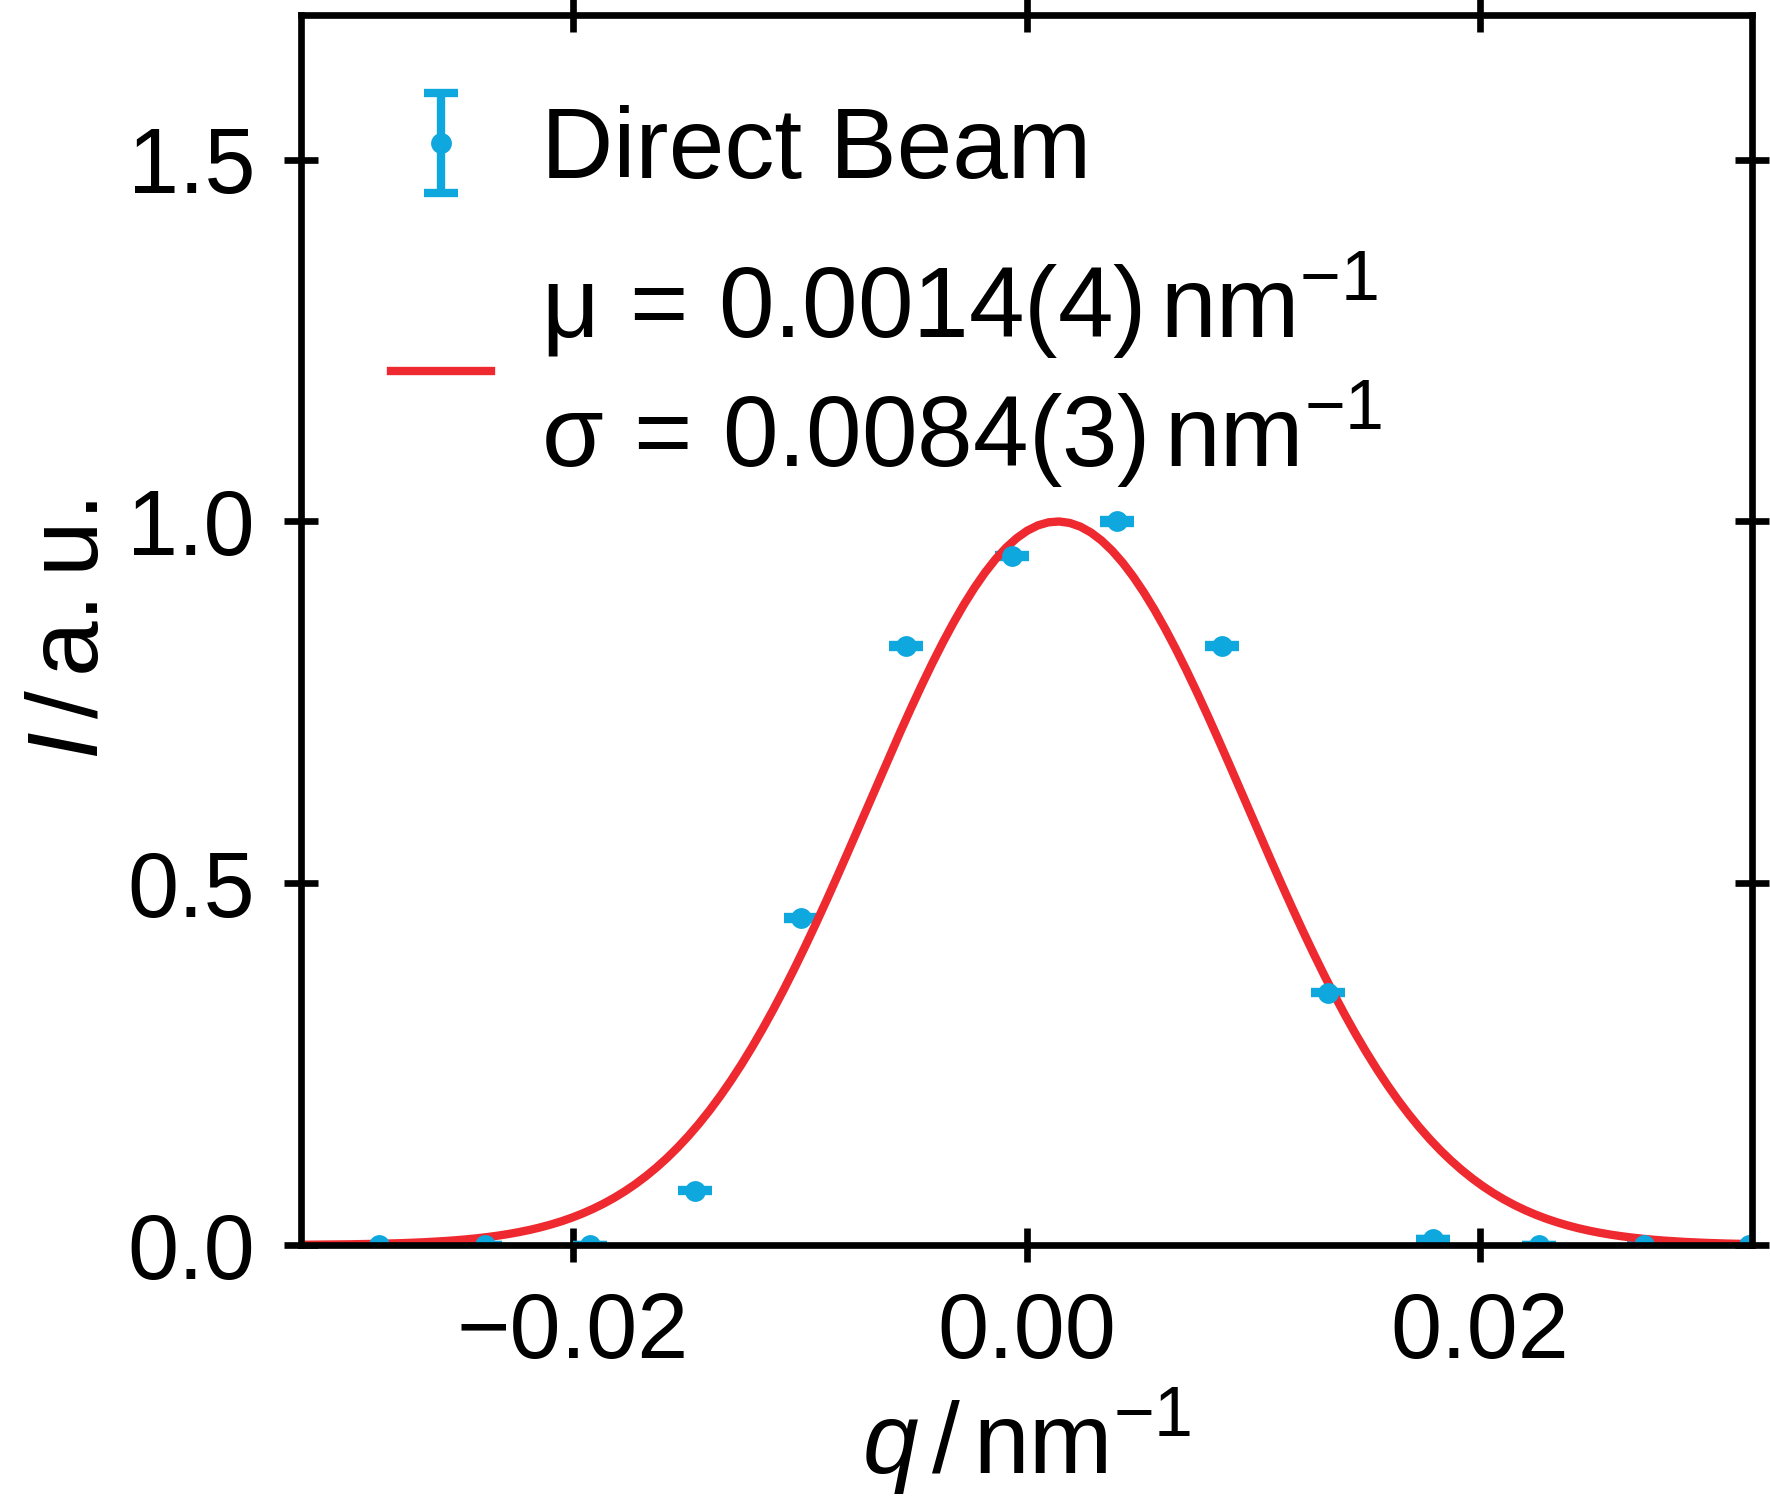
\includegraphics{appendix_instruments_GALAXIDirectBeam}
      \caption{\label{fig:appendix:lss:galaxi:directBeam}Direct beam width measured at GALAXI for slit widths of $s_2 \eq 0.5 \unit{mm}$ and $s_3 \eq 0.9 \unit{mm}$ with the detector set to a distance of $L \eq 1.73 \unit{m}$.}
    \end{figure}
\end{document}